Pengujian sistem navigasi berbasis \emph{layered costmap} dilakukan pada lingkungan simulasi Mujoco yang diadaptasi dari arena Kontes Robot SAR Indonesia (KRSRI) 2024. Tujuan pengujian adalah untuk memvalidasi kinerja setiap komponen sistem navigasi, yaitu lokalisasi ICP, \emph{global planner} A*, dan \emph{local planner} DWA, dalam skenario yang merepresentasikan kondisi pasca gempa. Pengujian dilakukan pada tiga region (A, B, C) dengan variasi kondisi lantai dan konfigurasi parameter untuk mengevaluasi efektivitas dan keterbatasan pendekatan yang diusulkan.

\subsection{Pengujian Lokalisasi ICP}

Pengujian lokalisasi ICP bertujuan untuk mengukur akurasi estimasi pose robot pada berbagai kondisi lantai dan region. ICP menggunakan prekomputasi KNN dengan tabel \emph{hash} (\emph{lookup} $O(1)$) yang dikonfigurasi dengan $K = 8$ dan radius pencarian $r = 10$ sel. Setiap iterasi ICP melakukan \emph{subsampling} \emph{scan} dengan \emph{random stride}, pencocokan titik menggunakan KNN, pembobotan, dan estimasi transformasi optimal melalui \emph{SVD solver}. Proses diulang hingga konvergen atau mencapai batas iterasi maksimum. Kecepatan gerak robot selama pengujian lokalisasi ditetapkan sebesar $0,025$ m/s agar diperoleh data \emph{scan} yang cukup padat untuk proses \emph{scan matching}.

Metrik yang dievaluasi meliputi error estimasi pose pada sumbu $x$, sumbu $y$, dan $\theta$ (\emph{yaw}) di sepanjang lintasan robot. Pengujian dilakukan pada tiga skenario utama:

\begin{figure}[H]
\centering
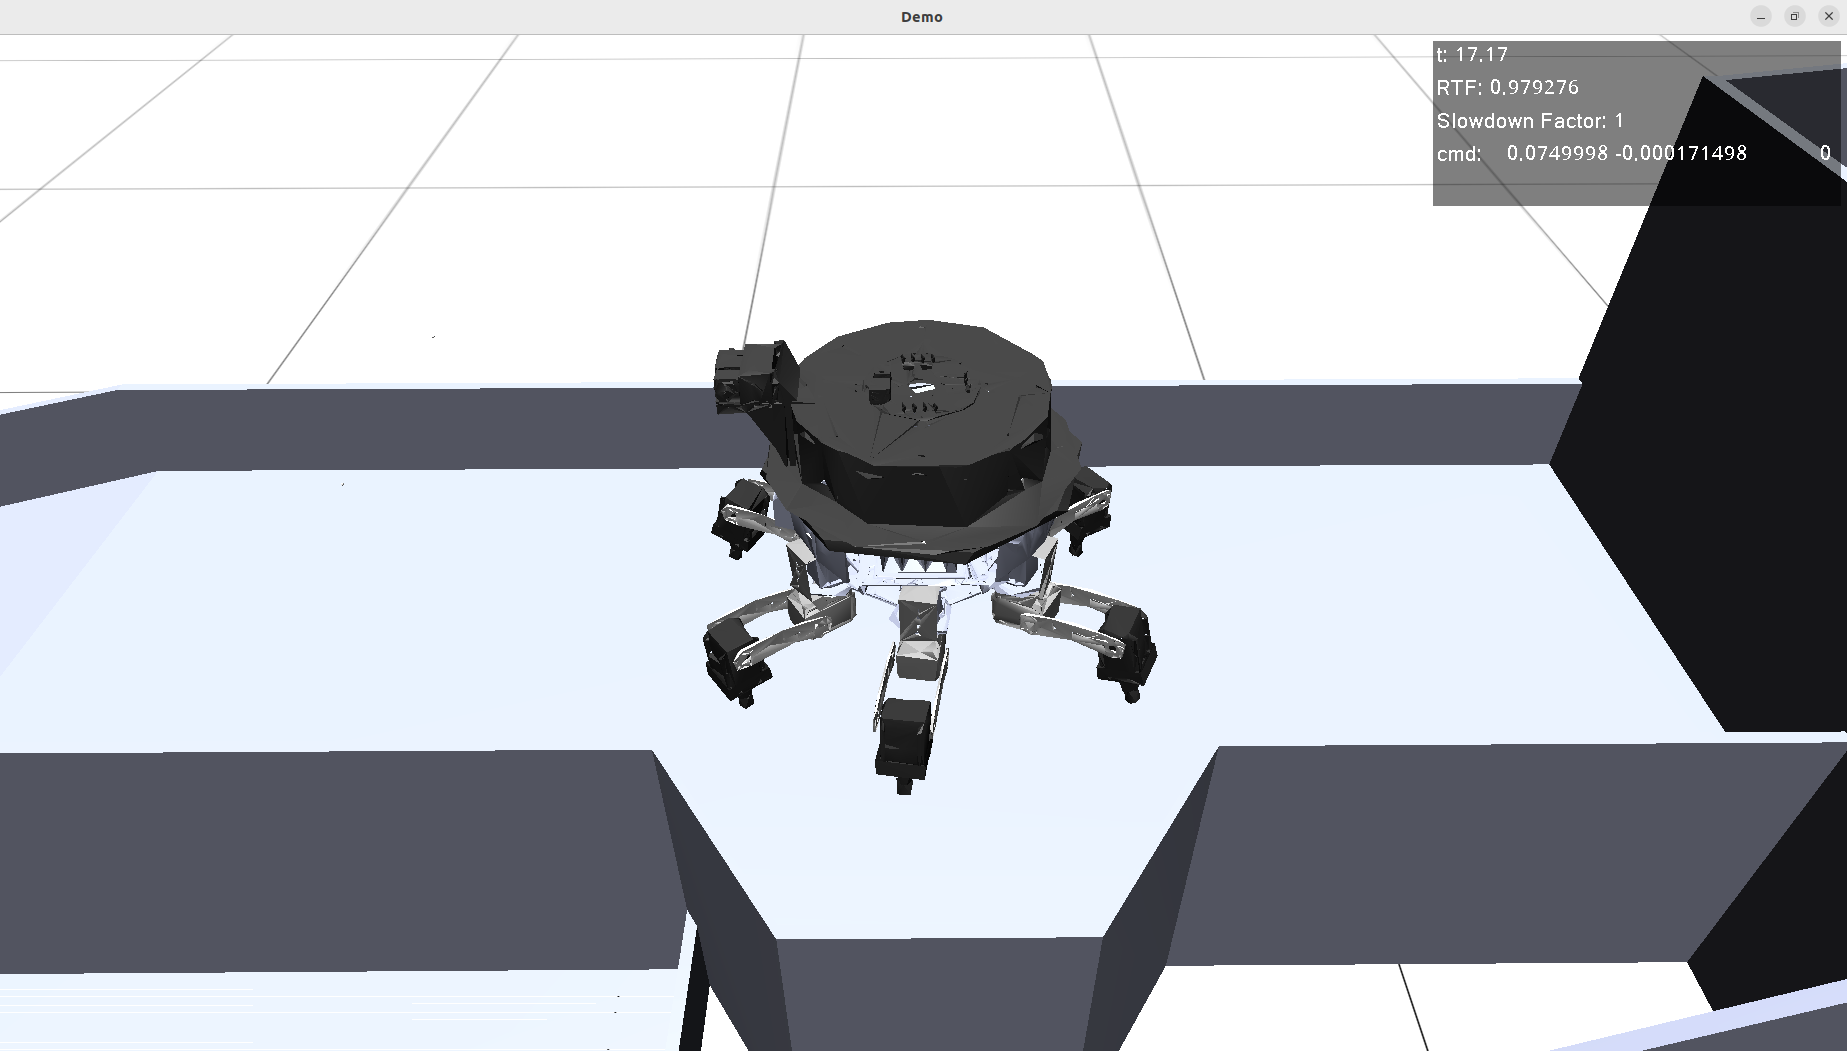
\includegraphics[width=0.7\textwidth]{gambar/sim_RA.png}
\caption{Simulasi di Region A}
\label{fig:sim_ra}
\end{figure}

\begin{figure}[H]
\centering
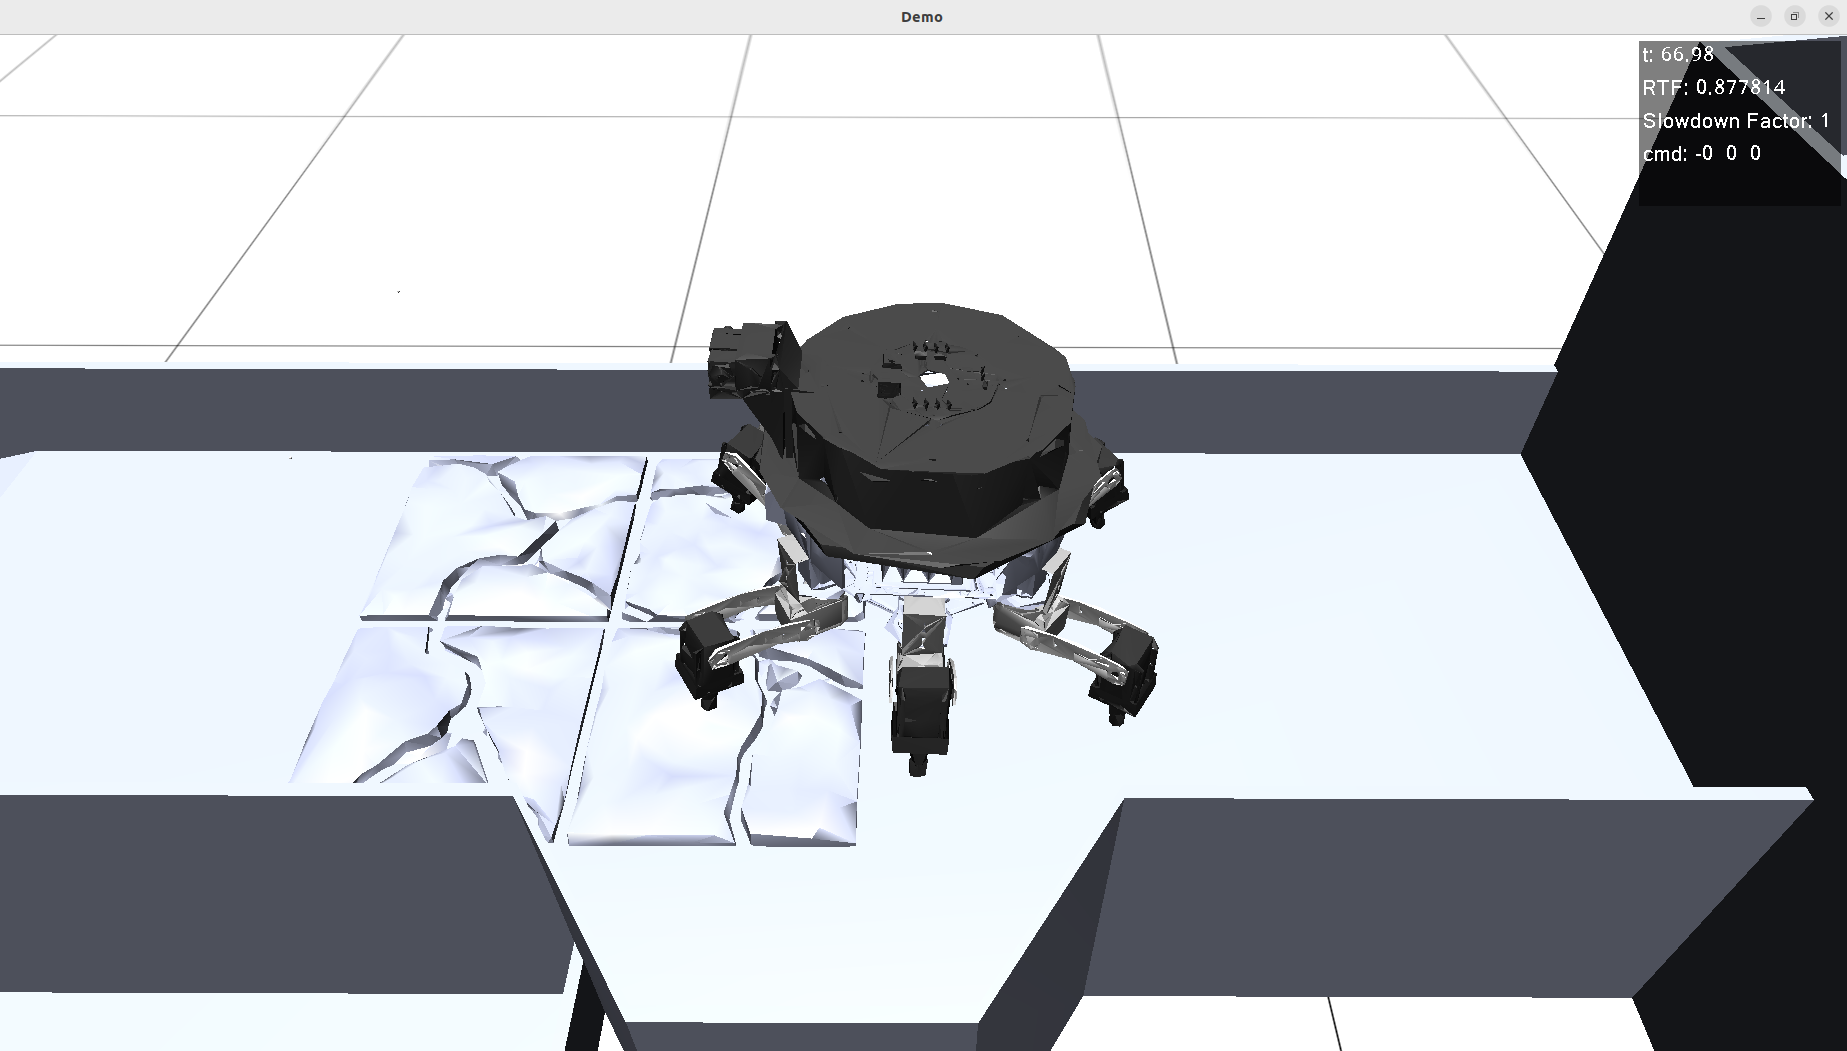
\includegraphics[width=0.7\textwidth]{gambar/sim_RA_rough.png}
\caption{Simulasi di Region A dengan rintangan lantai}
\label{fig:sim_ra_rough}
\end{figure}

\begin{figure}[H]
\centering
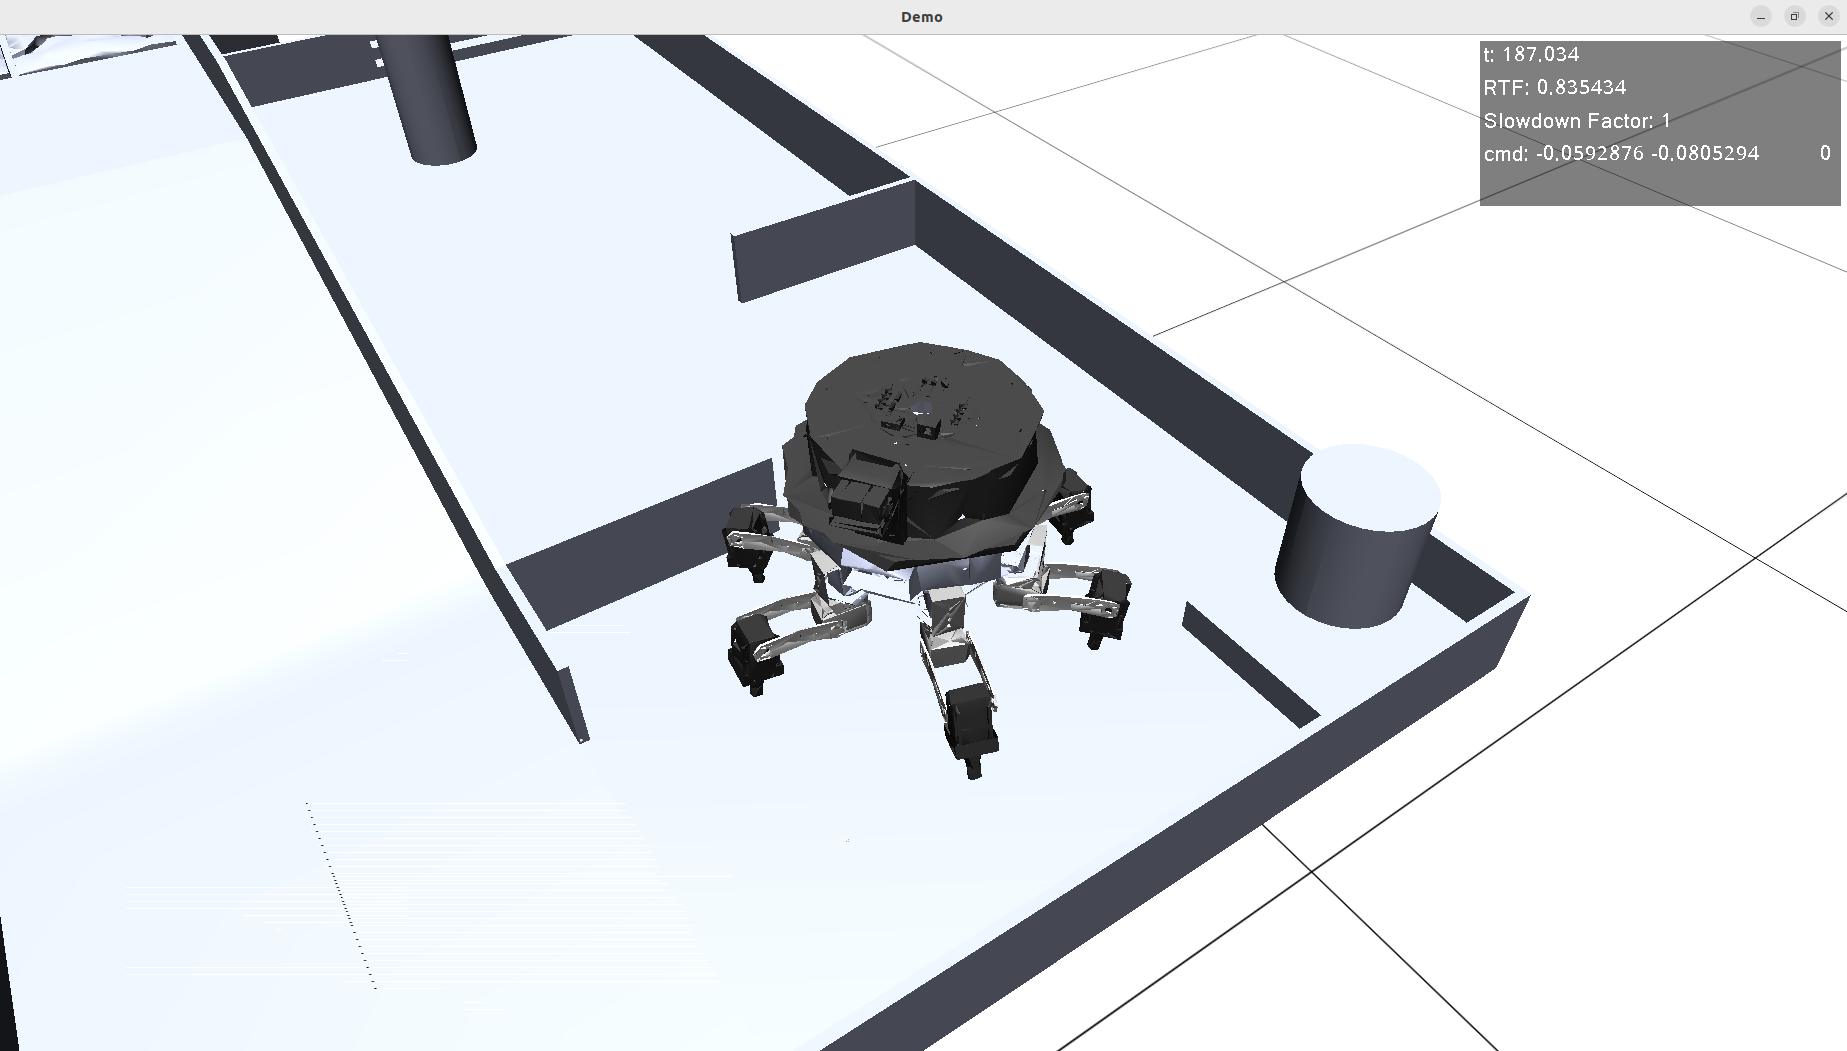
\includegraphics[width=0.7\textwidth]{gambar/sim_RC2.png}
\caption{Simulasi di Region C}
\label{fig:sim_rc2}
\end{figure}

\subsection{Pengujian Global Planner (A*)}

Pengujian \emph{global planner} bertujuan untuk mengevaluasi pengaruh \emph{Cost Scaling Factor} (CSF) terhadap \emph{path} yang dihasilkan oleh algoritma A*. CSF memengaruhi kemiringan gradien biaya inflasi di sekitar \emph{obstacle} sebagaimana dijelaskan pada persamaan fungsi inflasi. Global planner menggunakan \emph{cost function} dengan parameter \emph{cost factor} $f = 0.55$, \emph{neutral cost} $c_{\text{neutral}} = 1$, dan \emph{lethal cost} $c_{\text{lethal}} = 253$.

Pengujian dilakukan pada seluruh tiga region (A, B, C) dengan masing-masing empat variasi nilai CSF: 10, 20, 50, dan 100. Metrik evaluasi yang digunakan meliputi:

\begin{enumerate}
    \item Panjang \emph{path} yang dihasilkan (m).
    \item Waktu komputasi yang diperlukan untuk perencanaan \emph{path} (ms).
    \item \emph{Minimum clearance} terhadap \emph{obstacle} terdekat (m).
    \item Jumlah \emph{waypoint} penyusun \emph{path}.
    \item \emph{Cross track error} terhadap \emph{ground truth}, mencakup nilai rata-rata (\emph{mean}), maksimum (\emph{max}), dan simpangan baku (\emph{standard deviation}) (m).
\end{enumerate}

Hasil dari keempat nilai CSF pada setiap region dibandingkan untuk menentukan pengaruh CSF terhadap karakteristik \emph{path} dan menentukan nilai CSF yang paling sesuai untuk masing-masing region.

\subsection{Pengujian Local Planner (DWA)}

Pengujian \emph{local planner} DWA bertujuan untuk mengevaluasi kemampuan algoritma DWA dalam mengikuti \emph{global path} yang telah direncanakan sebelumnya. DWA bekerja dengan melakukan \emph{sampling} semua kemungkinan kecepatan $(v_x, v_y, \omega)$ dalam \emph{dynamic window}, mensimulasikan setiap sampel menjadi \emph{trajectory}, dan memilih \emph{trajectory} dengan skor terendah berdasarkan tujuh kriteria penilaian: \emph{oscillation cost}, \emph{obstacle cost}, \emph{goal front cost}, \emph{alignment cost}, \emph{path cost}, \emph{goal cost}, dan \emph{twirling cost}.

Konfigurasi \emph{velocity sampling} yang digunakan adalah $N_{v_x} = 6$, $N_{v_y} = 6$, dan $N_{\omega} = 30$, sehingga total terdapat $1080$ \emph{trajectory} yang dievaluasi setiap siklus kendali.

Batas kecepatan pada setiap \emph{region} dikonfigurasi secara berbeda sesuai dengan karakteristik medan:

\begin{table}[H]
\centering
\caption{Konfigurasi batas kecepatan DWA per region}
\label{tab:dwa_speed_limits}
\begin{tabular}{lcccc}
\toprule
\textbf{Region} & \textbf{max $v_x$} & \textbf{min $v_x$} & \textbf{max $v_y$} & \textbf{min $v_y$} \\
\midrule
A & 0,08 & 0,05  & 0,08 & $-0,08$ \\
B & 0,08 & 0,05  & 0,08 & $-0,08$ \\
C & 0,025 & $-0,025$ & 0,025 & $-0,025$ \\
\bottomrule
\end{tabular}
\end{table}

Pada Region A dan B yang memiliki area lebih luas, robot dapat bergerak dengan kecepatan yang lebih tinggi. Sementara itu, Region C yang memiliki area lebih sempit dan \emph{trajectory} yang lebih kompleks dibatasi dengan kecepatan yang lebih rendah untuk menjaga stabilitas navigasi.

Pengujian dilakukan pada dua skenario navigasi penuh dari Region A menuju Region C:

\begin{enumerate}
    \item \textbf{Kondisi normal}: Seluruh \emph{obstacle} telah diketahui oleh \emph{global path}.
    \item \textbf{Kondisi gempa}: Terdapat \emph{obstacle} yang tidak diketahui oleh \emph{global path} dan baru terdeteksi oleh sensor LiDAR saat navigasi berlangsung.
\end{enumerate}

Metrik yang digunakan adalah waktu tempuh, serta \emph{mean cross track error} dan \emph{max cross track error} terhadap \emph{global path}.
